\documentclass[conference]{IEEEtran}
\IEEEoverridecommandlockouts
\usepackage[utf8]{inputenc}
\usepackage[T1]{fontenc}
\usepackage{mathptmx}
\usepackage[spanish,es-nodecimaldot,es-noshorthands,es-tabla]{babel}
\usepackage{cite}
\usepackage{amsmath}
\usepackage{graphicx}
\usepackage{textcomp}
\usepackage{xcolor}
\usepackage{booktabs}
\usepackage{url}
\renewcommand\IEEEkeywordsname{Palabras clave}
\newcommand{\pend}[1]{\textcolor{red}{[#1]}}
\setlength{\textfloatsep}{8pt plus 2pt minus 2pt}
\setlength{\intextsep}{8pt plus 2pt minus 2pt}

\begin{document}

\title{Las ganancias sobre oclusión sintética no anticipan\\la robustez a la oclusión real en la detección de personas}

\author{\IEEEauthorblockN{Celia Patricia Apaza Hilasaca, Brayan Raul Condori Quispe, Jhan Logan Ramos Quispe}
\IEEEauthorblockA{Universidad Peruana Unión (UPeU), Juliaca, Perú}}

\maketitle

\begin{abstract}
El aumento sintético de oclusión se usa para que los detectores de personas resistan la visibilidad parcial, pero su beneficio suele medirse con la misma oclusión artificial con que se entrena. Preguntamos si se transfiere a la oclusión real anotada por humanos. Comparamos un modelo base y otro con aumento, con los mismos datos e hiperparámetros, en 18 bloques que varían el oclusor (parches, siluetas, difusión, geometría real y orden de profundidad), el detector (YOLOv11 en dos tamaños, YOLO26s, RT-DETR-l, RetinaNet y Faster R-CNN), el dominio de entrenamiento y la cantidad de datos (117 corridas). Cada bloque tiene un control sintético y tres fuentes de oclusión real, de día y de noche, y sus hipótesis y reglas se fijaron antes de entrenarlo. Una celda pasa si mejora al menos 2 puntos de AP@0.5 con un intervalo del 95\,\% que excluye el cero. Con detectores de una etapa y \emph{transformers}, los 13 controles pasan y de 39 celdas reales pasan 4, ninguna a la vez estable entre semillas y propia de las personas ocluidas; 24 descartan una ganancia de 2 puntos y, con exposición igual al entrenamiento, el efecto medio es nulo. Una sola combinación transfiere: Faster R-CNN, de dos etapas, con siluetas (NightOwls +3,3 y CityPersons +2,3). No lo hace con difusión ni con profundidad, ni RetinaNet, de una etapa y con la misma red base y receta, con siluetas. En Faster R-CNN, el mayor control (+20,4, difusión) no transfiere y uno menor (+14,7, siluetas) sí: la ganancia sintética no anticipa la real y no basta para afirmar robustez frente a la oclusión real.
\end{abstract}

\begin{IEEEkeywords}
detección de personas, oclusión, aumento de datos, transferencia, poca luz, hipótesis preespecificadas
\end{IEEEkeywords}

\section{Introducción}
La detección de personas apoya la seguridad pública, la vigilancia y la robótica móvil, casi siempre con cámaras RGB convencionales. La oclusión, causa importante de fallos en la detección de peatones~\cite{Dollar2012}, y la baja iluminación~\cite{Loh2019} suelen coincidir de noche. En nuestros datos, un YOLOv11s ajustado sobre ExDark cae de 0,82 de AP@0.5 en personas sin oclusión a 0,24 en personas con oclusión severa.

Un remedio extendido es el \emph{aumento sintético de oclusión}: durante el entrenamiento se borran o se cubren partes de la persona~\cite{Zhong2020,Shang2018synthocc,Chi2020pedhunter}. Su beneficio suele medirse sobre la misma oclusión artificial o dentro del conjunto de entrenamiento, y rara vez sobre personas \emph{realmente} ocluidas por un auto, un poste u otra persona. Si no pasa a la oclusión real, los bancos de prueba sintéticos sobreestiman la robustez.

\textbf{Brecha.} En la literatura revisada (sección~II) no encontramos un estudio que (i) mida la transferencia a la oclusión real anotada con un control sintético que confirme que el aumento se aprendió, (ii) lo haga con varias fuentes reales independientes, (iii) ponga a prueba explicaciones alternativas (oclusor, detector, dominio, volumen de datos, exposición) con experimentos controlados y (iv) fije hipótesis y reglas antes de ver los resultados.

\textbf{Objetivos y contribución.} Los objetivos son medir la degradación por oclusión (OE1), el efecto del aumento sobre la oclusión sintética y la real según el oclusor (OE2), el detector (OE3) y el dominio y los datos (OE4), y su mecanismo (OE5)\footnote{La correspondencia entre objetivos, método, evidencia y pendientes, y todo el material citado como «suplemento», están en el material suplementario.}. Aportamos (1) evidencia controlada en 18 bloques con cinco tipos de oclusor y seis detectores (de una y dos etapas y \emph{transformer}), incluido el único caso de transferencia (Faster R-CNN con siluetas) y dos pruebas preespecificadas que lo acotan; (2) un recuento único, con intervalos y separado por exposición al entrenamiento, que muestra que la ganancia sintética no anticipa la real; y (3) un protocolo de evaluación reutilizable: control sintético, varias fuentes reales, exposición igual y regla fijada de antemano.

\section{Trabajos relacionados y marco explicativo}
\textbf{Detección con oclusión y poca luz.} Los detectores recientes atacan la oclusión con cambios de arquitectura y reportan ganancias dentro de un mismo banco: PRNet++ refina anclas desde las partes visibles y evalúa subconjuntos de oclusión en CityPersons, Caltech y ECP-night~\cite{Song2022prnet}; MLFFCSP fusiona características de varios niveles con Random Erasing~\cite{Huan2023mlffcsp}. Para la conducción nocturna, un YOLOX con transferencia de dominio (datos diurnos degradados y nocturnos) sube el mAP 5,9 puntos sin estratificar por oclusión~\cite{Yi2022yolox}; POP-YOLOv8~\cite{Liu2026pop} y BNE-DETR~\cite{Li2026bne} reportan métricas agregadas.

\textbf{El aumento como señal de entrenamiento y como prueba.} Random Erasing~\cite{Zhong2020} inspiró variantes para peatones evaluadas dentro de CityPersons o CrowdHuman~\cite{Shang2018synthocc,Chi2020pedhunter}, y Copy-Paste pega objetos recortados sin modelar el contexto~\cite{Ghiasi2021copypaste}, antecedente directo de nuestros oclusores con orden de profundidad. Tres trabajos marcan el contraste. Kassaw et al.\ encuentran que la oclusión sintética \emph{ordena} de forma parecida a la real a clasificadores ya entrenados~\cite{Kassaw2026occl}: sirve para comparar modelos. Taori et al.\ muestran que la robustez ganada frente a cambios sintéticos casi no pasa a cambios naturales, salvo con datos más amplios y diversos~\cite{Taori2020shifts}, y Pytel et al.\ que, en estimación de pose, el aumento de oclusión no resuelve la oclusión~\cite{Pytel2021tilting}. Nosotros preguntamos si la ganancia producida por un aumento de oclusión en detección, medida sobre oclusión sintética, anticipa la ganancia sobre oclusión real.

\textbf{Alternativas estructurales y marco explicativo.} Las redes composicionales representan el objeto por partes y son más robustas a la oclusión parcial que el aumento de datos~\cite{Kortylewski2020compnet,Wang2020compnet}; WALT aprende representaciones amodales a partir de oclusión real en cámaras fijas~\cite{Reddy2022walt}, y la adaptación de dominio ataca la brecha nocturna desde los datos~\cite{Yi2022yolox,Song2022prnet}. Nuestro estudio no evalúa esas vías: se limita al aumento a nivel de píxel sobre imágenes RGB para la detección modal. Como marco explicativo usamos el aprendizaje por atajos~\cite{Geirhos2020shortcut}: una red puede reducir su pérdida aprendiendo los rasgos del oclusor artificial sin aprender a detectar personas incompletas, y los detectores de peatones ya generalizan mal entre conjuntos~\cite{Hasan2021elephant,Sukesh2024camped}. La revisión partió de tres búsquedas en Scopus exportadas el 13/10/2026 (155, 8 y 71 registros; cadenas en el suplemento), de las que salieron los cinco artículos semilla~\cite{Song2022prnet,Reddy2022walt,Huan2023mlffcsp,Sukesh2024camped,Yi2022yolox}, y se completó con búsquedas dirigidas en Crossref y arXiv.

\section{Método}
\textbf{Diseño, hipótesis y regla.} Es un experimento controlado: en cada bloque, el modelo base (V1) y el aumentado (V3) comparten datos, hiperparámetros, aumento base y máquina; V3 añade el aumento de oclusión solo en el entrenamiento. Todas las hipótesis de transferencia predicen que el déficit persiste (no hay transferencia). Se \emph{confirma} esa predicción si menos de dos de las tres fuentes reales \emph{pasan}, es decir, mejoran el AP@0.5 al menos +2 puntos porcentuales (pp, media de semillas) con un IC del 95\,\% por imágenes que excluye el cero, y el control sintético sí pasa; si no pasa el control, el bloque no es concluyente. H11 predecía lo contrario (una ganancia en las personas más ocluidas), H16a y H16b que la transferencia de Faster R-CNN se extendería a otros oclusores, y H13 un orden de realismo. El planteamiento original incluía además un módulo de atención (variantes V2 y V4; H1, H2 y H5), sin ganancia en oclusión real (suplemento). Cada hipótesis, su regla y su código se fijaron con una huella criptográfica SHA-256 antes de entrenar su bloque y ninguna se reformuló; la huella prueba que nada cambió desde la fecha registrada por el proyecto, pero no hubo registro externo. La tabla de hipótesis, huellas, fechas y primera corrida está en el suplemento. La pregunta se reorientó tras el primer experimento y H9b--H17 se diseñaron viendo resultados previos y revisiones: el programa es adaptativo.

\textbf{Datos.} ExDark~\cite{Loh2019}, con la partición de Cui et al.~\cite{Cui2021}, tiene 2\,658 imágenes con personas y 7\,460 instancias; 1\,183 de esas imágenes se usan para entrenar. Fuentes de oclusión real: (1) NightOwls~\cite{Neumann2019}, de noche, con el atributo de oclusión de sus autores (530 peatones ocluidos de validación; hasta 20\,000 fotogramas de entrenamiento); (2) CityPersons~\cite{Zhang2017}, de día, partición oficial \emph{heavy} (visibilidad 20--65\,\%, 733 instancias); (3) un indicador sobre ExDark que estima la oclusión entre personas por el solapamiento de sus cajas (101 instancias severas), que se correlaciona poco con la visibilidad anotada (Spearman 0,24). La gradación visual manual se descartó como referencia ($\kappa$ de 0,06 a 0,60). Los tres conjuntos se usan bajo sus licencias de investigación no comercial y sus imágenes no se redistribuyen.

\textbf{Aumento y control.} Familias de oclusor: parches opacos o con textura; siluetas recortadas de objetos y personas reales; oclusores pintados por Stable Diffusion 1.5 con diez objetos de COCO~\cite{Rombach2022ldm}; siluetas colocadas con patrones de visibilidad reales de CityPersons; y recortes de objetos delante de la persona según la profundidad monocular de Depth Anything V2~\cite{Yang2024depthv2}. En V3 se ocluyen 1--3 personas por imagen con cobertura de 0,30 a 0,85. El \emph{control} de cada familia aplica su mismo generador a todas las personas de ExDark test con cobertura de 0,70 a 1,00, con imágenes y oclusores no vistos en el entrenamiento (bancos de recortes disjuntos o generaciones nuevas). Mide si el aumento se aprendió; para saber si mide algo más que el propio oclusor, evaluamos cada familia en el control de las demás (matriz cruzada).

\textbf{Detectores y exposición.} YOLOv11s, YOLOv11m~\cite{Ultralytics2024}, YOLO26s~\cite{Ultralytics2026yolo26} (SGD, tasa 0,002, lote 16), RT-DETR-l~\cite{Zhao2024rtdetr} (AdamW, $10^{-4}$) y, de torchvision con la misma red base ResNet-50 FPN, Faster R-CNN~\cite{Ren2017faster} y RetinaNet~\cite{Lin2017focal} (SGD, 0,01 y 0,005, lote 8), preentrenados en COCO~\cite{Lin2014}, entrada de 640 px, Ultralytics 8.4.143 (receta completa en el suplemento). En los primeros bloques cada variante se seleccionó por su mejor época en validación (paciencia 20, hasta 100 épocas), lo que dejó exposiciones \emph{desiguales}: en H4, H4-Y26, H6 y H8, V1 se eligió en las épocas 1--51 y V3 en las 31--89. Desde H9b, V1 y V3 se entrenan un número fijo de épocas y se evalúan con los últimos pesos; esos bloques son la evidencia primaria. Máquinas: una laptop con NVIDIA GeForce RTX 5050 Laptop (8 GB) y, para H11, H12 y H14--H17, una RTX 4090 alquilada.

\textbf{Evaluación.} AP@0.5 de la clase \emph{person} por estrato de oclusión, con las instancias de otros estratos como regiones \emph{ignore}, como en CityPersons~\cite{Zhang2017}. IC por \emph{bootstrap} de percentiles sobre imágenes (1\,000 réplicas)~\cite{Efron1993} y, como sensibilidad, jerárquico sobre semillas e imágenes (2\,000). El umbral de +2 pp es el efecto mínimo de interés: supera la desviación típica entre semillas del AP de V1 en las fuentes reales (mediana 1,5 pp). Una celda \emph{descarta} una ganancia relevante si el límite superior de su IC es menor que +2 (prueba unilateral de no superioridad~\cite{Lakens2017tost}). La tasa de fallos MR$^{-2}$~\cite{Dollar2012} y AP@0.5:0.95 son secundarias (suplemento).

\begin{table*}[t]
\caption{Bloques, hipótesis y resultados: cambio del AP@0.5 (pp) de V3 frente a V1, media de 3 semillas. Exp.: exposición al entrenamiento, igual (I, épocas fijas), desigual (D, selección por validación) o temprana en ambas (T). NO: NightOwls ocluidos; CP: CityPersons \emph{heavy}; EX: indicador de ExDark, severa. * pasa (+2 pp con IC por imágenes $>0$). Confirmada: se confirma la predicción de no transferencia. IC de cada celda en el suplemento.}
\label{tab:res}
\centering
\footnotesize
\setlength{\tabcolsep}{4pt}
\begin{tabular}{@{}llllcrrrrl@{}}
\toprule
\textbf{Bloque} & \textbf{Detector} & \textbf{Entrenamiento} & \textbf{Oclusor} & \textbf{Exp.} & \textbf{Control} & \textbf{NO} & \textbf{CP} & \textbf{EX} & \textbf{Veredicto} \\
\midrule
H3 & YOLOv11s & ExDark & Parches & T & $+60{,}92$* & $-3{,}17$ & $-0{,}36$ & $-3{,}25$ & No confirmada (predecía ganancia) \\
H4 & YOLOv11s & ExDark & Siluetas & D & $+10{,}63$* & $-16{,}79$ & $-3{,}94$ & $-5{,}02$ & Refutada (predecía ganancia) \\
H4-Y26 & YOLO26s & ExDark & Siluetas & D & $+12{,}01$* & $-14{,}31$ & $-4{,}42$ & $-3{,}51$ & Mismo patrón \\
H6 & YOLOv11s & CityPersons & Siluetas & D & $+23{,}74$* & $-1{,}35$ & $+1{,}82$ & $+0{,}94$ & Confirmada (0 de 3) \\
H7 & YOLOv11s & NightOwls 20\,000 & Siluetas & D & --- & $-1{,}43$ & $-3{,}94$ & $-9{,}15$ & Confirmada \\
H8 & RT-DETR-l & ExDark & Siluetas & D & $+10{,}97$* & $-6{,}98$ & $-3{,}47$ & $-2{,}21$ & Confirmada (0 de 3) \\
H9 & YOLOv11s & ExDark & Difusión & T & $+2{,}60$* & $-1{,}93$ & $+1{,}23$ & $+2{,}82$* & Confirmada (1 de 3) \\
H9b & YOLOv11s & ExDark & Difusión & I & $+15{,}23$* & $+0{,}01$ & $+1{,}52$ & $-3{,}03$ & Confirmada (0 de 3) \\
H10 & YOLOv11s & ExDark & Geometría real & I & $+18{,}39$* & $-2{,}05$ & $+2{,}37$* & $-4{,}88$ & Confirmada (1 de 3) \\
H10-s & YOLOv11s & ExDark & Siluetas & I & $+10{,}99$* & $-1{,}12$ & $+2{,}26$* & $-3{,}50$ & (brazo de comparación de H10) \\
H11 & YOLOv11s & CityPersons & Siluetas & I & $+24{,}66$* & $+1{,}95$ & $+1{,}31$ & $-2{,}44$ & No confirmada (predecía ganancia) \\
H12a & YOLOv11m & ExDark & Siluetas & I & $+14{,}45$* & $-0{,}39$ & $+0{,}25$ & $+3{,}04$ & Confirmada (0 de 3) \\
H12b & YOLOv11m & ExDark & Difusión & I & $+19{,}04$* & $+0{,}78$ & $+1{,}11$ & $-0{,}56$ & Confirmada (0 de 3) \\
H14 & YOLOv11s & ExDark & Profundidad & I & $+7{,}42$* & $-1{,}50$ & $-0{,}16$ & $+5{,}49$* & Confirmada (1 de 3) \\
H15 & Faster R-CNN & ExDark & Siluetas & I & $+14{,}72$* & $+3{,}28$* & $+2{,}33$* & $-1{,}00$ & Refutada (2 de 3) \\
H16a & Faster R-CNN & ExDark & Difusión & I & $+20{,}35$* & $+0{,}92$ & $-0{,}76$ & $+0{,}80$ & Refutada (predecía transferencia) \\
H16b & Faster R-CNN & ExDark & Profundidad & I & $+9{,}63$* & $+0{,}37$ & $+0{,}60$ & $-0{,}45$ & Refutada (predecía transferencia) \\
H17 & RetinaNet & ExDark & Siluetas & I & $+6{,}60$* & $-2{,}11$ & $-0{,}28$ & $-3{,}77$ & Confirmada (0 de 3) \\
\bottomrule
\end{tabular}
\end{table*}

\section{Resultados}
\textbf{Recuento.} Todas las cifras son V3$-$V1 en AP@0.5 (tabla~\ref{tab:res}). En los 13 bloques comparables con detectores de una etapa y \emph{transformers} (todos salvo H7, sin control, y los cuatro de torchvision, añadidos después del recuento), los 13 controles pasan, de +2,6 a +60,9 pp. De las 39 celdas reales pasan 4: el indicador de ExDark en H9 (+2,82) y en H14 (+5,49), que no resisten el intervalo jerárquico, y CityPersons en H10 (+2,37) y en su brazo de siluetas (+2,26), donde las personas sin oclusión ganan más (+5,3). Otras 24 celdas descartan una ganancia de +2 pp (19 con el intervalo jerárquico). Sin el indicador de ExDark pasan 2 de 26 celdas y ningún bloque alcanza dos fuentes. Con H15--H17 son 17 controles que pasan y 6 de 51 celdas reales, 29 de las cuales descartan +2 pp.

\textbf{La exposición explica el daño, no la ausencia de ganancia.} Con exposición igual (21 celdas de H9b a H14), el efecto medio es $+0{,}02$ pp, pasan 3 celdas y 3 son negativas con IC (con las 12 de H15--H17, $+0{,}01$ en 33); con exposición desigual (12 celdas de H4, H4-Y26, H6 y H8), el efecto medio es $-4{,}94$ pp y 6 son negativas con IC. El daño grande de las siluetas en NightOwls ($-16{,}8$ en H4) se reduce a $-1{,}12$ con épocas fijas (H10-s): refleja el sobreajuste al dominio de la regla de selección. Lo que se mantiene en ambos casos es que no hay ganancia.

\textbf{Detector, dominio y datos.} El patrón se repite con RT-DETR-l (H8), YOLO26s y YOLOv11m (H12), que aprende el aumento con más fuerza que YOLOv11s (controles +14,45 y +19,04) y no lo transfiere a ninguna fuente. Con Faster R-CNN (H15), en cambio, el control sube +14,72 y pasan NightOwls (+3,28 [+1,64; +4,79]) y CityPersons (+2,33 [+1,01; +3,69]), ambas también con el intervalo jerárquico: H15 se refuta. En NightOwls mejoran más las personas sin oclusión (+4,37) que las ocluidas, pero en CityPersons las ocluidas ganan más (\emph{heavy} +2,33, \emph{partial} +2,57) que las visibles (\emph{bare} +0,88); en ExDark no cambia nada, y la tasa de fallos baja menos de 2 pp. Las dos pruebas preespecificadas para acotarlo fallan: con difusión y con profundidad (H16a y H16b), Faster R-CNN aprende el aumento (+20,35 y +9,63) y no lo transfiere (0 de 3, ninguna celda real por encima de +0,92), y RetinaNet con siluetas (H17), que solo difiere en ser de una etapa, tampoco (0 de 3; baja en todos los estratos reales, más en las personas visibles). Una V1 de Faster R-CNN re-entrenada en otra máquina cambió $-1{,}92$ pp en CityPersons y +3,42 en ExDark: la variación entre máquinas es del orden de las ganancias de H15. Re-entrenar en CityPersons (H6) quita el signo negativo, pero el control gana +23,74 y \emph{heavy} +1,82; con épocas fijas y semillas nuevas, la ganancia sobre las personas más ocluidas (visibilidad 0,20--0,50) es +1,44 [$-$0,64; +3,34]: H11 no se confirma. Con 20\,000 imágenes de NightOwls (H7), $-1{,}43$ [$-$3,98; +1,00].

\textbf{Oclusor, geometría y profundidad.} Ni los oclusores por difusión (H9, H9b), ni la geometría real (H10; frente a las siluetas simples, $-0{,}93$, +0,10 y $-1{,}38$ pp), ni los objetos colocados delante de la persona según la profundidad (H14) cumplen la regla. Con cinco semillas, CityPersons \emph{heavy} con siluetas resiste el intervalo jerárquico (+2,06 [+0,26; +4,17]), pero las personas sin oclusión mejoran el doble. En la matriz cruzada, cada familia gana también en los controles de las demás: pasan 13 de 20 celdas cruzadas (por ejemplo, las siluetas suben +15,8 en el control de geometría y la profundidad +11,7), y solo los parches se quedan casi en su propio control (+0,8 a +3,0 en los demás). El control no mide la memoria de unos oclusores concretos, sino una adaptación general a la oclusión sintética, que tampoco se transfiere a la real.

\begin{figure}[t]
\centering
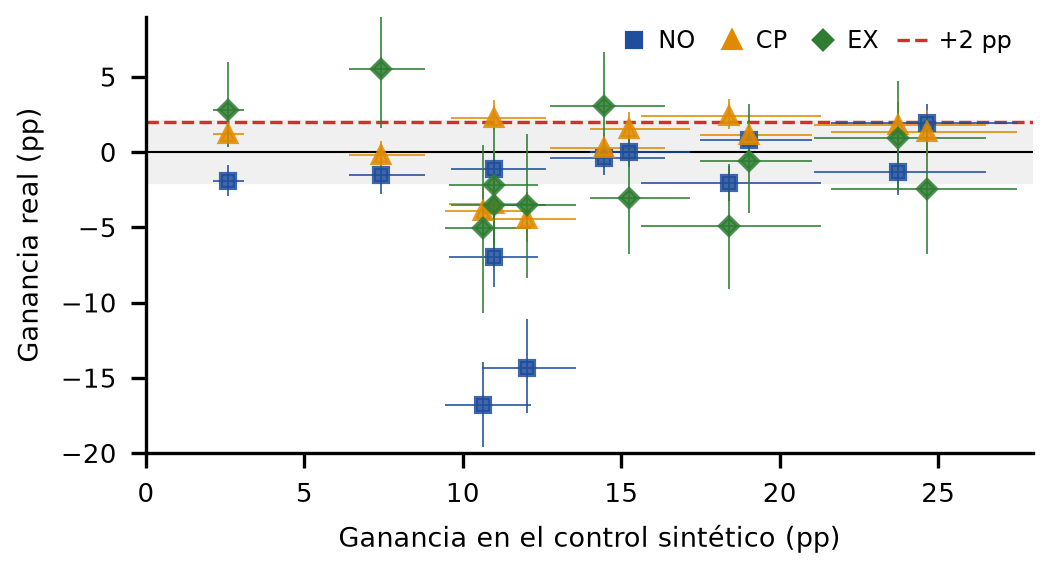
\includegraphics[width=\columnwidth]{fig_dispersion_es.png}
\caption{Ganancia en el control sintético frente a la ganancia en cada fuente real, con IC del 95\,\% por imágenes (13 bloques, 39 celdas; H3, con +60,9 en el control, queda fuera de escala: NO $-3{,}17$, CP $-0{,}36$, EX $-3{,}25$). Banda gris: $\pm2$ pp. $\rho$ de Spearman con IC \emph{bootstrap} de bloques: NO +0,41 [$-$0,18; +0,85], CP +0,30 [$-$0,26; +0,71], EX $-0{,}15$ [$-$0,67; +0,54].}
\label{fig:disp}
\end{figure}

\textbf{Capacidad predictiva y realismo (análisis posteriores).} Entre bloques no hay una asociación fiable entre la ganancia sintética y la real (fig.~\ref{fig:disp}); en un modelo mixto con intercepto por bloque, una desviación típica de ganancia sintética (14 pp) se asocia con +0,11 pp de ganancia real [$-$1,74; +1,95]. Con 13 bloques no se descarta una asociación moderada en NightOwls. Para medir el realismo (H13), un clasificador lineal sobre características de DINOv2~\cite{Oquab2024dinov2} separa 400 personas realmente ocluidas de CityPersons de las ocluidas con cada familia con AUC de 0,935 a 0,993, y de las mismas personas sin ocluir con 0,876; CLIP~\cite{Radford2021clip} coincide. La distancia KID~\cite{Binkowski2018kid}, que compara distribuciones, deja a siluetas, geometría y difusión algo más cerca de la oclusión real que las personas sin ocluir (características DINOv2 sin normalizar, 400 por conjunto: 1,57, 1,42 y 1,33 frente a 1,75), con intervalos que se solapan; medida solo sobre la región ocluida, ninguna familia se acerca al oclusor real (KID 2,5--3,4, frente a 3,6 sin oclusor y 0,01 entre dos mitades de oclusores reales). Lo que sí ayudó a las personas muy ocluidas fueron los datos anotados del dominio: entrenar en CityPersons lleva su \emph{heavy} a 0,59, frente a 0,24 como máximo sin entrenar allí; OWLv2~\cite{Minderer2023owlv2} y Grounding DINO~\cite{Liu2024gdino} sin ajuste no lo igualan.

\textbf{Mecanismo (exploratorio).} Con el aumento baja el \emph{recall} (exhaustividad) sobre los peatones ocluidos de NightOwls en todos los bloques con diagnóstico, y con siluetas y difusión bajan también los falsos positivos: los modelos detectan menos personas ocluidas, con más confianza.

\section{Discusión}
Los resultados coinciden con Taori et al.~\cite{Taori2020shifts} y Pytel et al.~\cite{Pytel2021tilting}: la robustez ganada frente a una perturbación sintética no pasa a la real, y lo que más ayudó fueron datos reales del dominio. No contradicen a Kassaw et al.~\cite{Kassaw2026occl}: la oclusión sintética puede ordenar modelos ya entrenados y aun así no anticipar cuánto ayuda un aumento entrenado con ella. Son compatibles con un atajo~\cite{Geirhos2020shortcut}: el modelo aprende el oclusor artificial, que sigue siendo distinguible de la oclusión real (H13), pero ese mecanismo no se ha probado de forma confirmatoria. Faster R-CNN con siluetas es la única excepción: con un control casi igual al de YOLOv11m (+14,72 frente a +14,45) transfiere en dos fuentes, y en CityPersons de forma propia de la oclusión. No es un efecto de las dos etapas ni de las siluetas por separado, porque no aparece con otros oclusores (H16) ni con RetinaNet (H17): depende de la combinación, y su tamaño es del orden de la variación entre máquinas. Lo que el control sintético no permite es saber de antemano qué combinación transferirá: dentro del mismo detector, el control más alto no transfiere. La conclusión se limita al aumento a nivel de píxel sobre RGB; no refuta las arquitecturas composicionales~\cite{Kortylewski2020compnet,Wang2020compnet}, la supervisión amodal~\cite{Reddy2022walt} ni la adaptación de dominio~\cite{Yi2022yolox}.

\textbf{Limitaciones.} \emph{De arquitectura:} seis detectores, con YOLOv11 en dos tamaños; un solo detector de dos etapas, con una red base y un conjunto de entrenamiento, y las corridas de una V1 en dos máquinas difieren hasta 3,4 pp. \emph{De los datos:} CityPersons es diurna y NightOwls usa una cámara de vehículo, de modo que ninguna fuente reproduce la vigilancia fija en la oscuridad; el indicador de ExDark solo capta la oclusión entre personas y de él salen dos de las cuatro celdas que pasan; todo es AP@0.5 de una clase. \emph{Del protocolo de evaluación:} tres semillas por celda (cinco en la extensión); las 39 celdas comparten líneas base y conjuntos de prueba y no son pruebas independientes, sin corrección por multiplicidad; los primeros bloques tienen exposición desigual; la huella no tiene sello de tiempo de un tercero, y el realismo se midió en espacios de características y no de forma perceptual.

\textbf{Líneas futuras.} (1) Oclusión tomada de imágenes reales y supervisión amodal~\cite{Reddy2022walt}. (2) Adaptación de dominio para la noche~\cite{Yi2022yolox} y arquitecturas por partes~\cite{Wang2020compnet}. (3) Repetir el protocolo con video real de vigilancia nocturna anotado por visibilidad, con rastreo: ByteTrack~\cite{Zhang2022bytetrack} y BoT-SORT~\cite{Aharon2022botsort} sostienen la identidad durante una oclusión breve recuperando cajas de baja confianza, pero solo si el detector las emite, de modo que nuestro resultado concierne al detector que los alimenta. (4) Medir la velocidad en un dispositivo embebido. Para la práctica: un banco de oclusión sintética sirve como control de que un aumento funciona, pero afirmar robustez exige un conjunto, aunque sea pequeño, de oclusión real anotada del dominio de uso.

\section{Conclusión}
En 18 bloques con cinco tipos de oclusor, seis detectores, tres dominios de entrenamiento y hasta cinco semillas, el aumento sintético de oclusión mejoró siempre la detección sobre oclusión sintética. Sobre oclusión real, con exposición igual su efecto medio fue nulo, y solo una combinación, Faster R-CNN con siluetas, se transfirió en dos fuentes; el mismo detector con otros oclusores y RetinaNet con siluetas no. La ganancia sintética no anticipó qué combinación transferiría. Los datos anotados del dominio ayudaron mucho más a las personas ocluidas de ese dominio. La robustez a la oclusión debe evaluarse con oclusión real anotada y un control sintético.

\section*{Declaraciones}
\textbf{Datos y código.} Código, registros, huellas, listas de muestreo y suplemento en \url{https://github.com/jhanrq8888/argos-occlusion-transfer} (público); los pesos entrenados se depositarán con DOI en Zenodo al publicarse. \textbf{Financiamiento:} ninguno. \textbf{Conflicto de intereses:} ninguno. \textbf{Contribuciones (CRediT):} J.~L. Ramos Quispe: conceptualización, metodología, software, análisis formal, investigación, curación de datos y redacción del borrador; C.~P. Apaza Hilasaca: conceptualización, metodología (diseño del prerregistro), revisión y edición; B.~R. Condori Quispe: curación de datos, validación, visualización, revisión y edición. \textbf{Uso de IA:} los autores usaron Scopus AI (Elsevier) para apoyar la búsqueda de los artículos semilla, y Claude (Anthropic) para la búsqueda, el código de análisis y la redacción y edición del texto. Revisaron y verificaron el código, los resultados, las referencias y el texto, de los que asumen la responsabilidad.

\bibliographystyle{IEEEtran}
\bibliography{references}

\end{document}
